\section{Elastica minimization via graph-cuts}

\begin{frame}
\center
\huge
Elastica minimization via graph-cuts

\vspace{2em}

\begin{minipage}{0.7\textwidth}
\normalsize
\begin{itemize}
\item{Balance coefficient to estabilize curvature estimation.}
\item{Set up a graph whose minimum cut approximates the zero level set of the balance coefficient.}
\item{GraphFlow algorithm. Up to $10$x faster than FlipFlow.}
\end{itemize}
\end{minipage}

\end{frame}

\begin{frame}
{Non-submodular elastica}
{Balance coefficient}
\begin{minipage}{0.5\textwidth}
\center
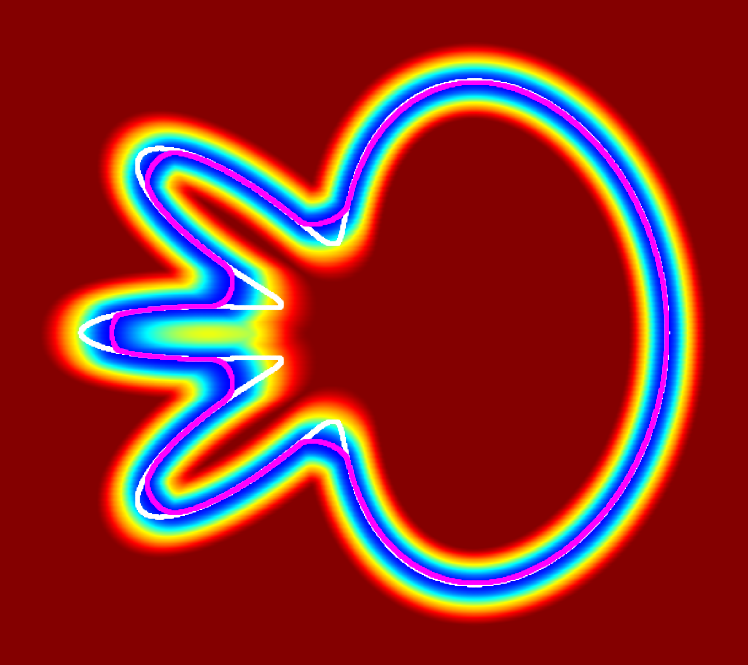
\includegraphics[scale=0.2]{figures/non-submodular-elastica/balance-coefficient-zero-level-set.png}
\end{minipage}
\begin{minipage}{0.49\textwidth}
\footnotesize
\begin{itemize}
\item{Balance coefficient}
\begin{align*}
u_r(D,p) &= \left( \frac{\pi r^2}{2} - |B_r(p) \cap D| \right)^2
\end{align*}
\item{White contour: contour of the shape}
\item{Pink contour: $\epsilon$-level set of the balance coefficient}
\end{itemize}
\end{minipage}
\end{frame}

\begin{frame}
{Elastica minimization via graph-cuts}
{Graph cut}
\center
\only<1>{
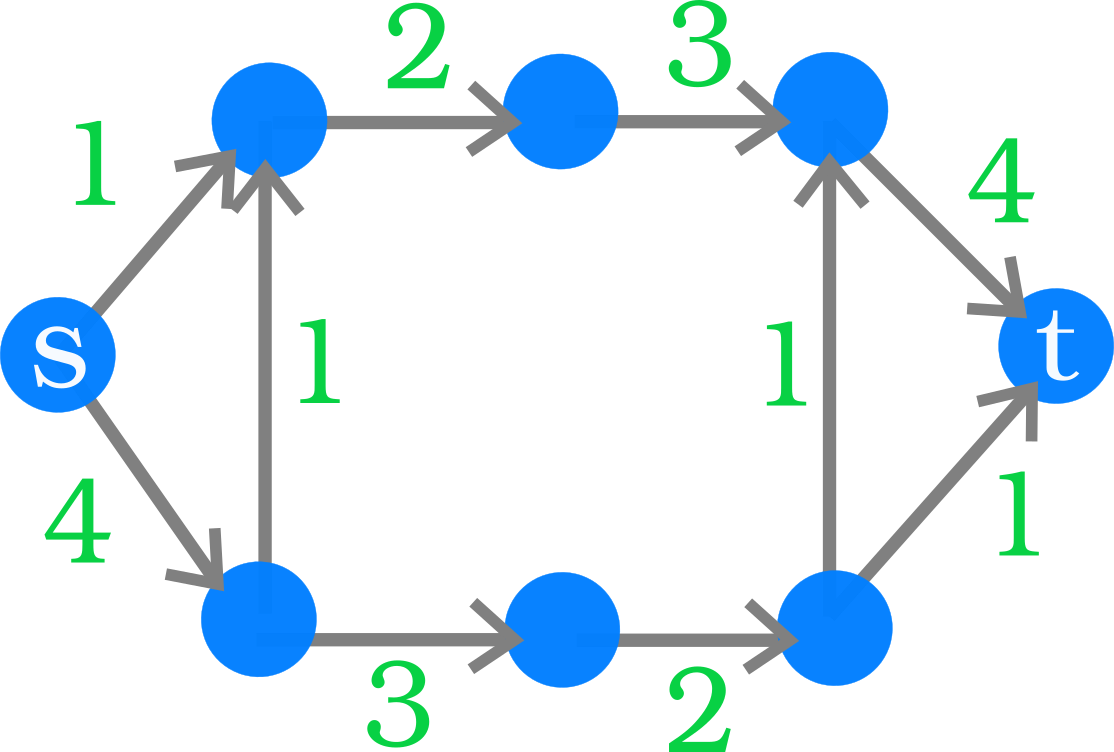
\includegraphics[scale=0.25]{figures/graphcut/cut-1.png}}%
\only<2>{
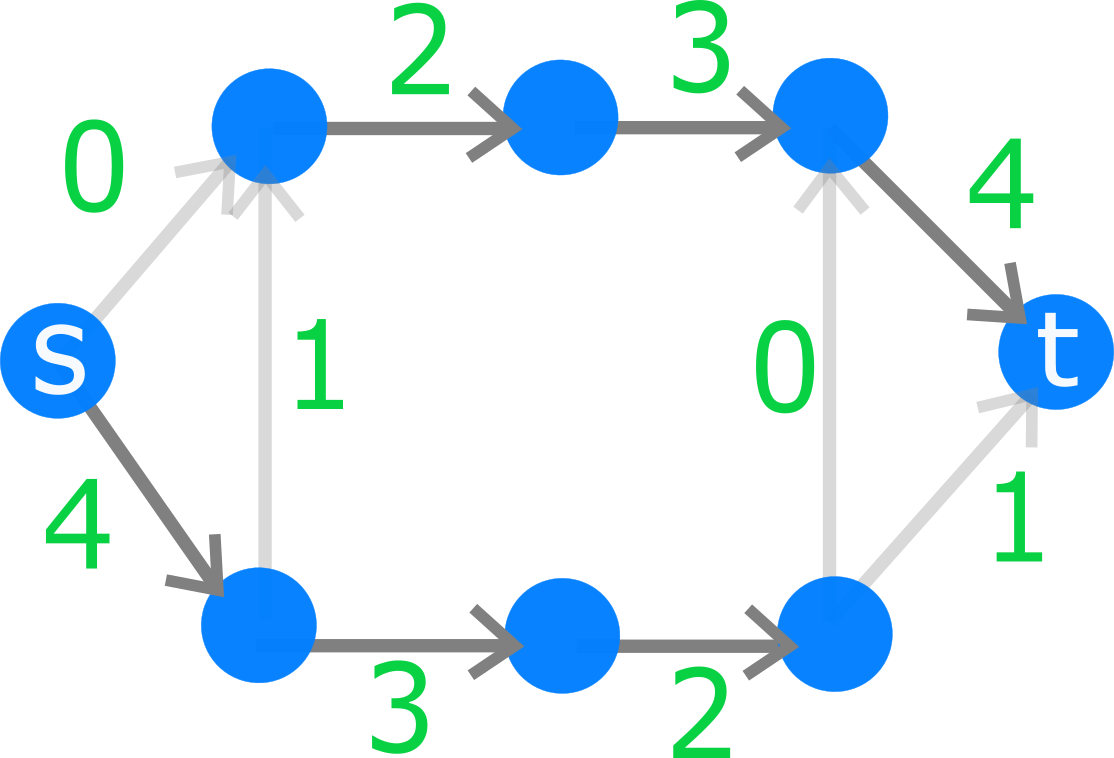
\includegraphics[scale=0.25]{figures/graphcut/cut-2.png}}%
\only<3>{
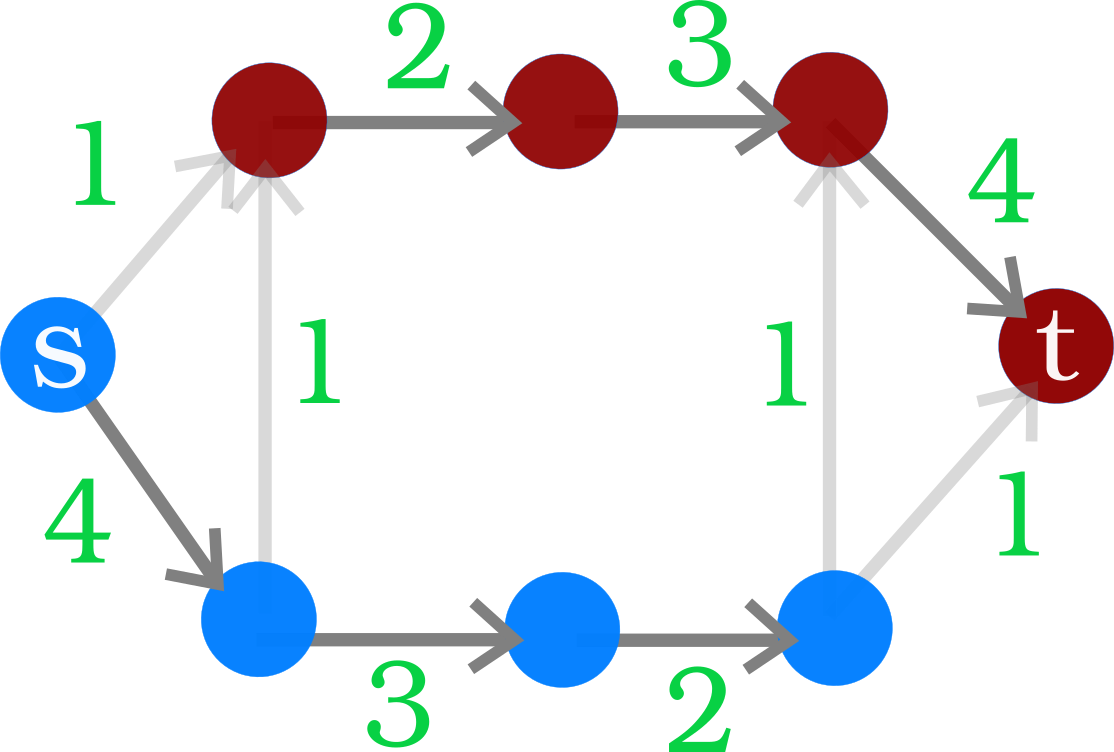
\includegraphics[scale=0.25]{figures/graphcut/cut-3.png}}%
\end{frame}


\begin{frame}
{Elastica minimization via graph-cuts}
{Building the graph}

\begin{minipage}{0.3\textwidth}
\only<1>{
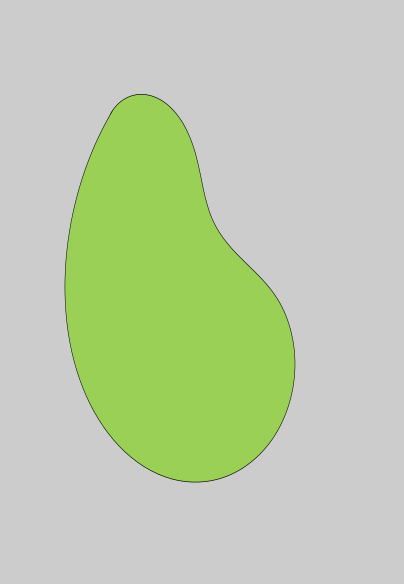
\includegraphics[scale=0.5]{figures/graphcut/graph-model-1.png}}%
\only<2-3>{
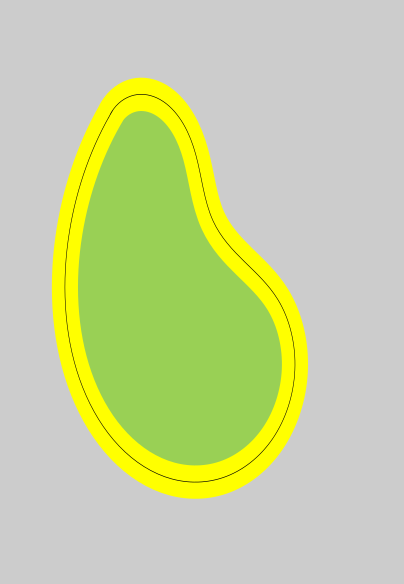
\includegraphics[scale=0.5]{figures/graphcut/graph-model-2.png}}%
\only<4->{
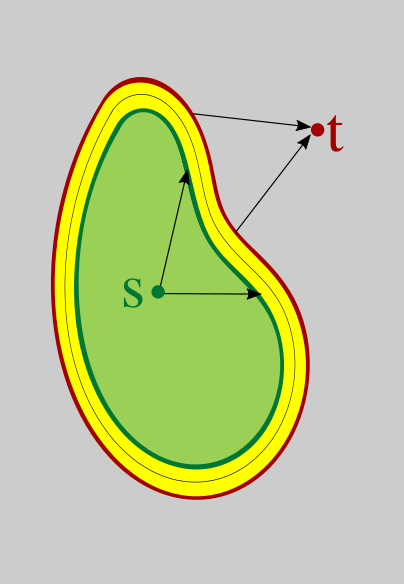
\includegraphics[scale=0.5]{figures/graphcut/graph-model-3.png}}%
\end{minipage}
%
%
\begin{minipage}{0.69\textwidth}
\footnotesize
\begin{itemize}
\onslide<2->{\item{Optimization band
\begin{align*}
%\only<2>{O_n(D) :=& \{ p \in D \; | \; -n \leq d_D(p) \leq n \} \\}
\only<2->{O(D) :=& \{ p \in D \; | \; -n \leq d_D(p) \leq n \} \\}
\onslide<3->{F(D) :=& D \setminus O(D)}
\end{align*}}}
\onslide<4->{\item{Graph $\mathcal{G}_D(\mathcal{V},\mathcal{E},c)$
\begin{align*}
\mathcal{V} &= \{ v_p \; | \; p \in O(D) \} \cup \{s,t\} \\
\highlight{6}{4,5,7-}{\mathcal{E}} &= \highlight{6}{4,5,7-}{\{ \{v_p,v_q\} \; | \; p,q \in O(D) \text{ and } q \in \mathcal{N}_4(p) \}} \cup \highlight{5}{4,6-}{\mathcal{E}_{st}} \\
\highlight{5}{4,6-}{\mathcal{E}_{st}} &= \highlight{5}{4,6-}{\{ (s,v_p), (v_p,t) \; | \; p \in O(D) \}}
\end{align*}}}
\onslide<7->{\item{Edge's weight
\begin{center}
\begin{tabular}{|c|c|}
\hline
\textbf{edge} $e$ & $\mathbf{c(e)}$\\
\hline
$\{v_p, v_q\}$ & $ \frac{1}{2}\left( u_r(D,p) + u_r(D,q)\right) $\\
\hline
$(s,v_p)$ & $M$\\
\hline
$(v_p, t)$ & $M$\\
\hline
\end{tabular}
\end{center}
}}
\onslide<8->{\item{Digital shape update
\begin{align*}
D^{(k+1)} &= F(D^{(k)}) + S^{(k)}
\end{align*}}}
\end{itemize}
\end{minipage}
\end{frame}
%
%
%
\begin{frame}
{Elastica minimization via graph-cuts}
{Shape evolution}

\begin{center}
$\alpha=1/8^2, \beta=1.$\\[1em]

\begin{tabular}{cc}
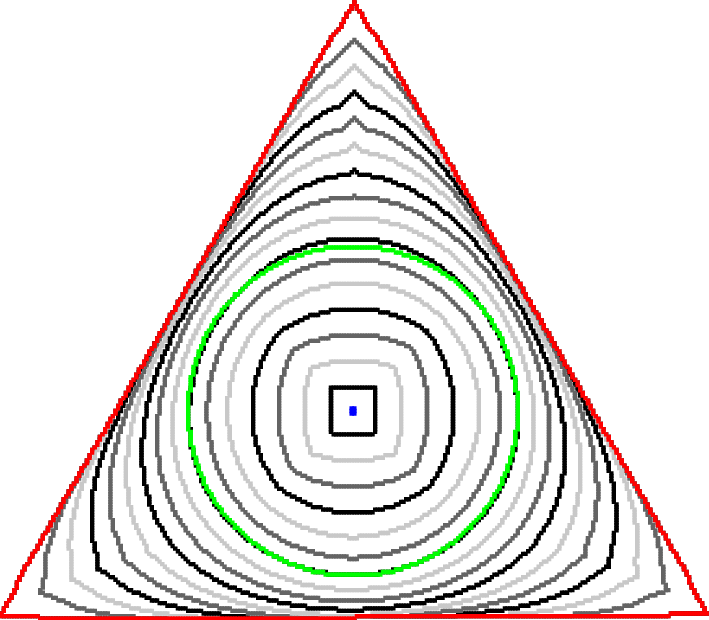
\includegraphics[scale=0.1]{figures/graphcut/no-neighborhood-flow-always-evolve/0.015625/triangle.png}\hspace{3em} &
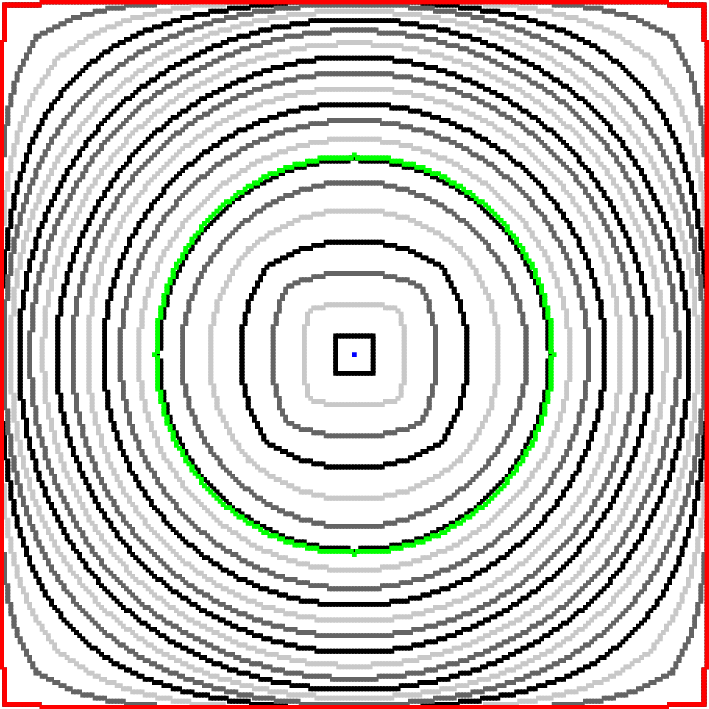
\includegraphics[scale=0.08]{figures/graphcut/no-neighborhood-flow-always-evolve/0.015625/square.png}\\[1em]
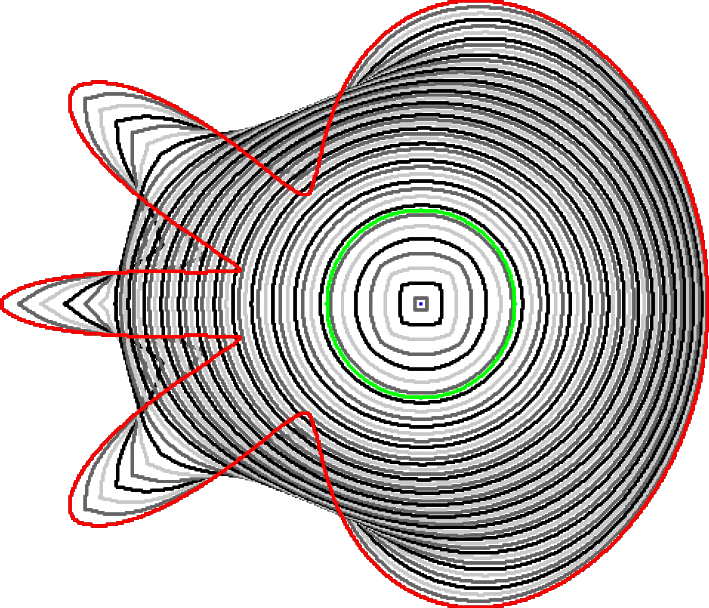
\includegraphics[scale=0.12]{figures/graphcut/no-neighborhood-flow-always-evolve/0.015625/flower.png}\hspace{3em} &
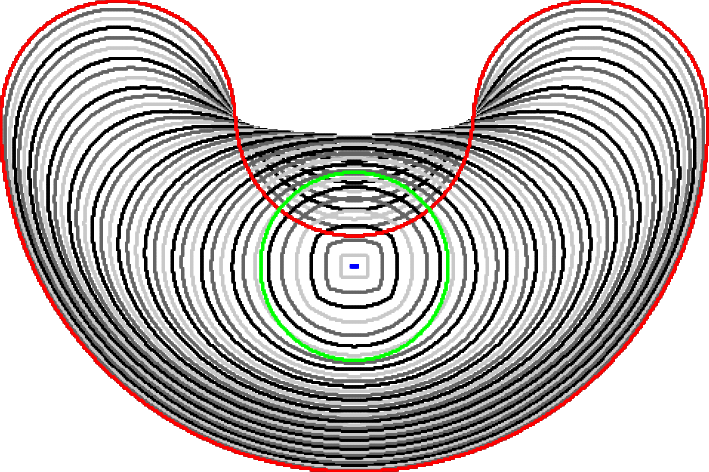
\includegraphics[scale=0.12]{figures/graphcut/no-neighborhood-flow-always-evolve/0.015625/bean.png}
\end{tabular}
\end{center}

\onslide<2->{
\begin{itemize}
\item{What if we stop the evolution when elastica increases?}
\end{itemize}}

\end{frame}

\begin{frame}
{Elastica minimization via graph-cuts}
{Shape evolution}

\begin{center}
Stop if elastica increases $(\alpha=1/8^2,\beta=1)$\\[1em]

\begin{tabular}{cc}
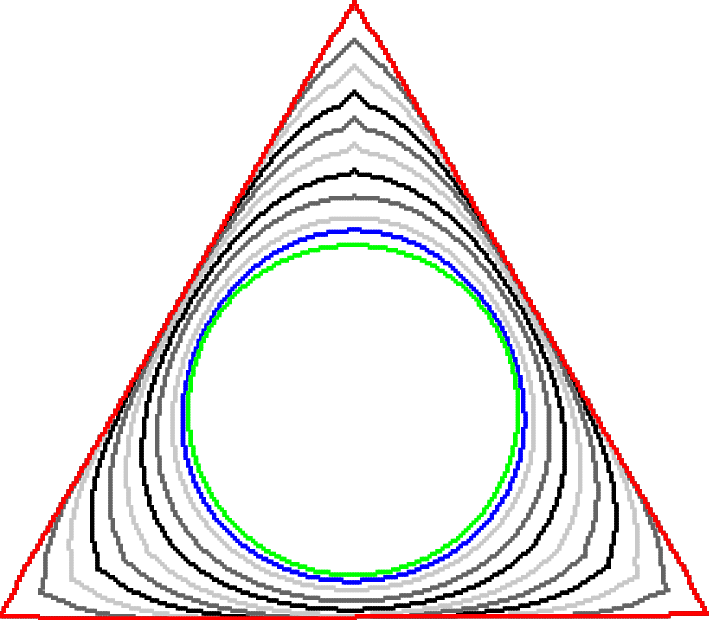
\includegraphics[scale=0.1]{figures/graphcut/no-neighborhood-flow-always-improve/0.015625/triangle.png}\hspace{3em} &
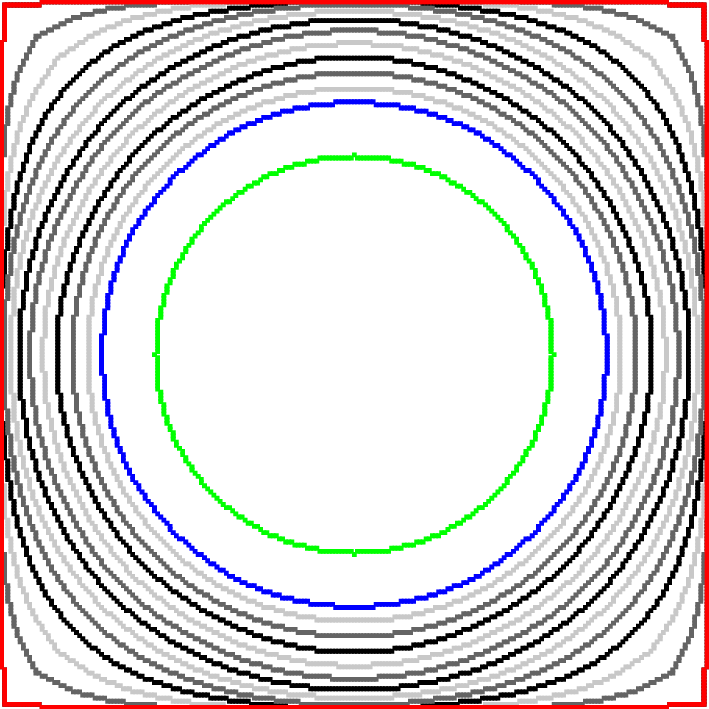
\includegraphics[scale=0.08]{figures/graphcut/no-neighborhood-flow-always-improve/0.015625/square.png}\\[2em]
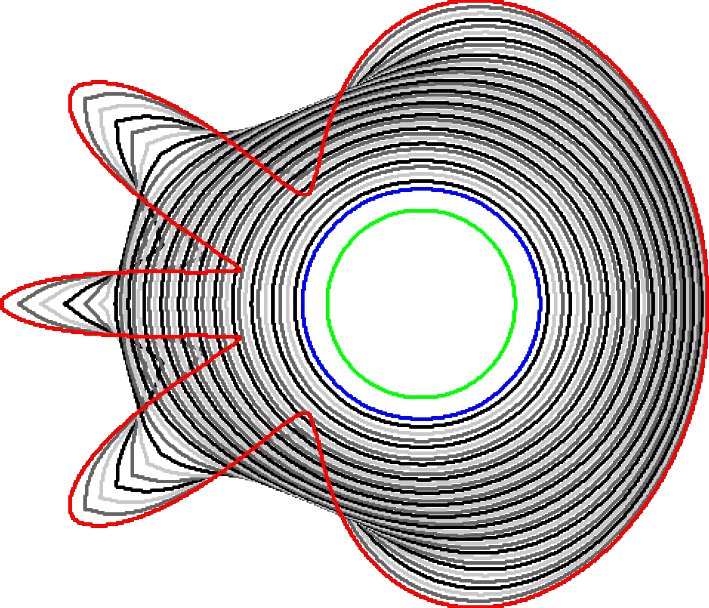
\includegraphics[scale=0.12]{figures/graphcut/no-neighborhood-flow-always-improve/0.015625/flower.png}\hspace{3em} &
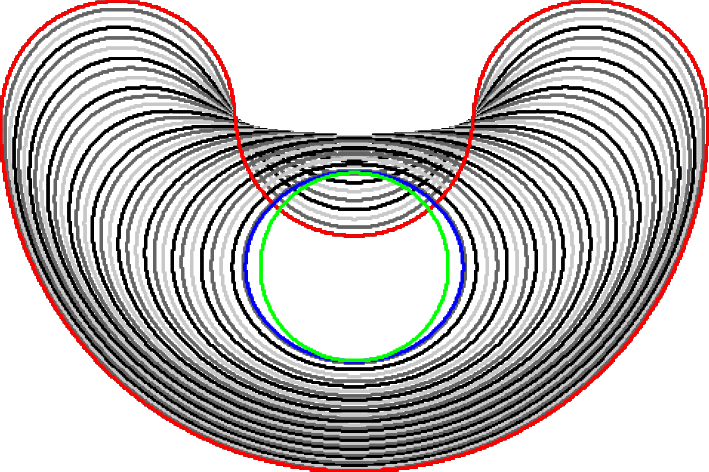
\includegraphics[scale=0.12]{figures/graphcut/no-neighborhood-flow-always-improve/0.015625/bean.png}
\end{tabular}

\end{center}




\end{frame}

\begin{frame}
{Elastica minimization via graph-cuts}
{Shape evolution}

\begin{center}
Stop if elastica increases $(\alpha=1/22^2,\beta=1)$\\[1em]

\begin{tabular}{cc}
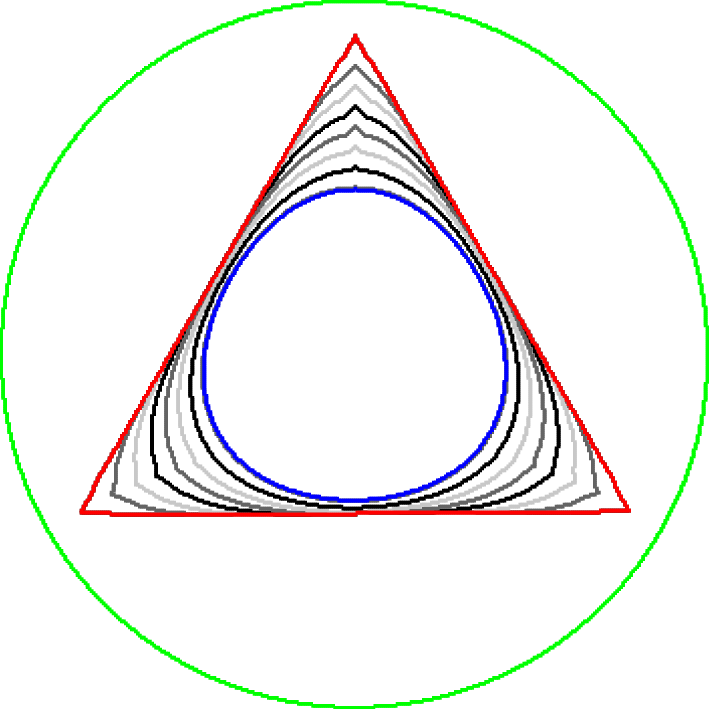
\includegraphics[scale=0.12]{figures/graphcut/no-neighborhood-flow-always-improve/0.0020661157/triangle.png}\hspace{3em} &
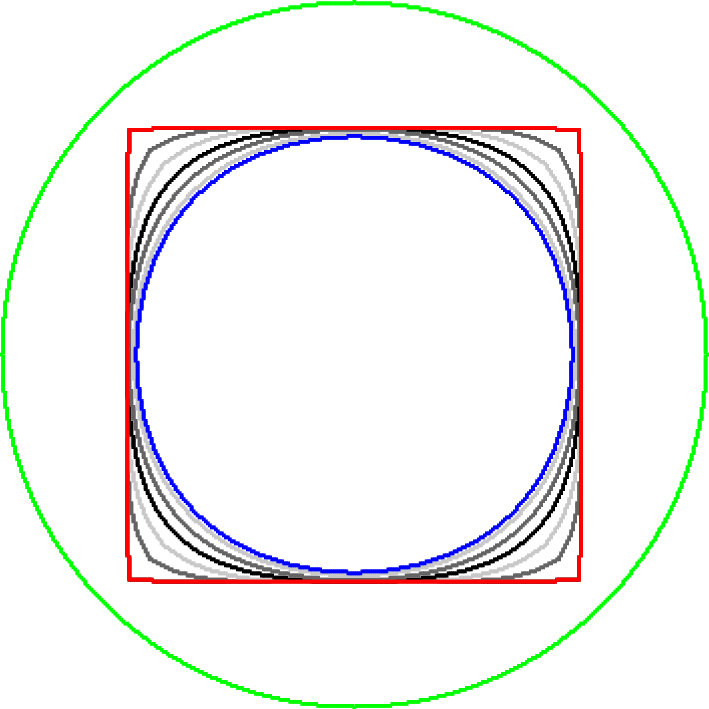
\includegraphics[scale=0.12]{figures/graphcut/no-neighborhood-flow-always-improve/0.0020661157/square.png}\\[2em]
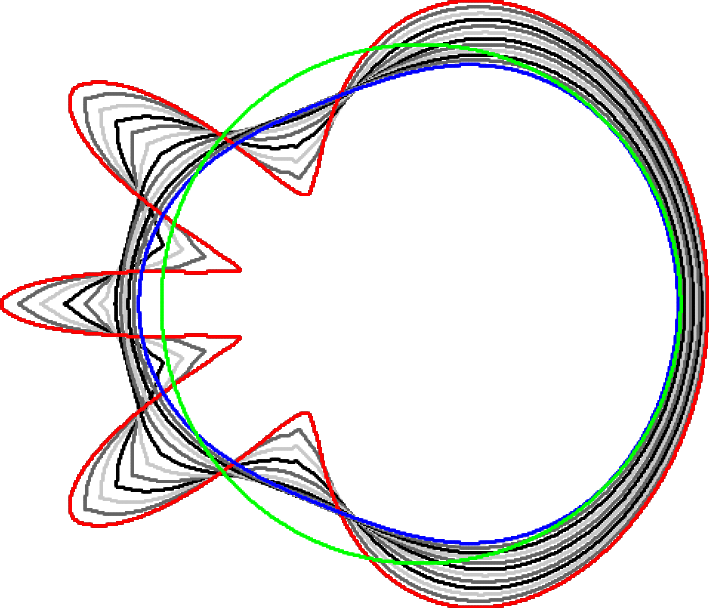
\includegraphics[scale=0.12]{figures/graphcut/no-neighborhood-flow-always-improve/0.0020661157/flower.png}\hspace{3em} &
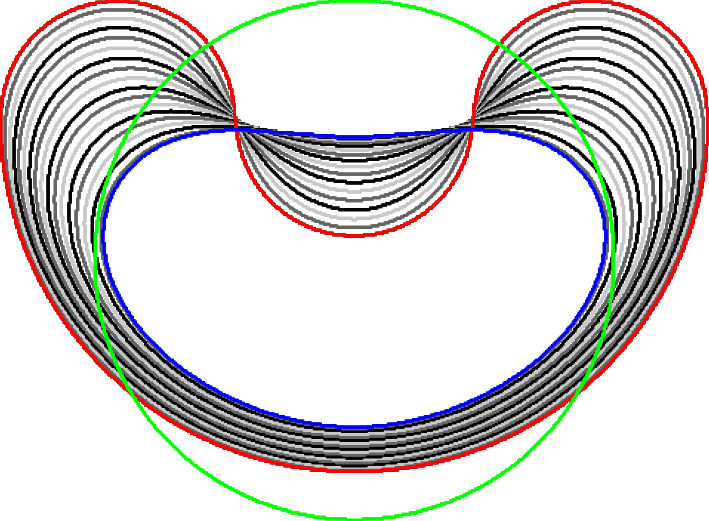
\includegraphics[scale=0.12]{figures/graphcut/no-neighborhood-flow-always-improve/0.0020661157/bean.png}
\end{tabular}

\end{center}




\end{frame}

\begin{frame}
{Elastica minimization via graph-cuts}
{The $a$-probe set}

\begin{definition}[$a$-probe set]
	Let $\Ds \subset \Omega \subset \mathbb{Z}^2$ a digital set and $a$ a natural number. The $a$-probe set of $\Ds$ is defined as
	\begin{align*}
		\mathcal{P}_a(\Ds) &= \Ds \cup \bigcup_{a' < a}{\Ds^{+a'} \cup \Ds^{-a'}},
	\end{align*}
	where $\Ds^{+a}$($\Ds^{-a}$) denotes a dilation(erosion) by a disk of radius $a$.
\end{definition}

\textbf{Candidate selection}
\[\begin{array}{l}
	sol(D^{(k)}) \longleftarrow \bigcup_{D' \in \mathcal{P}_a(D^{(k)})} \Big\{ F^{(k)} + S  \; | \; mincut(S,\mathcal{G}_{D'}) \Big\} 	
\end{array}
\]

\textbf{Candidate validation}
\[\begin{array}{l}
\Ds^{(k+1)} \longleftarrow \displaystyle \argmin_{ D' \in sol(D^{(k)}) }{ \hat{E}_{\vec{\theta}}(D')}
\end{array}
\]

\end{frame}

\begin{frame}
{Elastica minimization via graph-cuts}
{Shape evolution with $a$-probe set}

\center
\only<1>{Stop if elastica increases $(\alpha=1/22^2,\beta=1)$ \\[1em]}
\only<2>{Always update $(\alpha=1/22^2,\beta=1)$ \\[1em]}
\only<1>{
\begin{tabular}{cc}
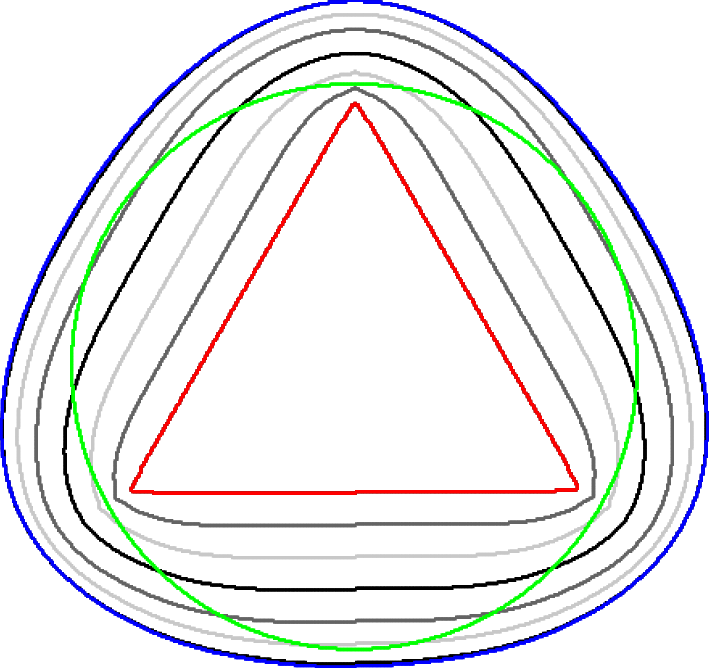
\includegraphics[scale=0.12]{figures/graphcut/with-neighborhood-flow-always-improve/triangle.png}\hspace{3em} &
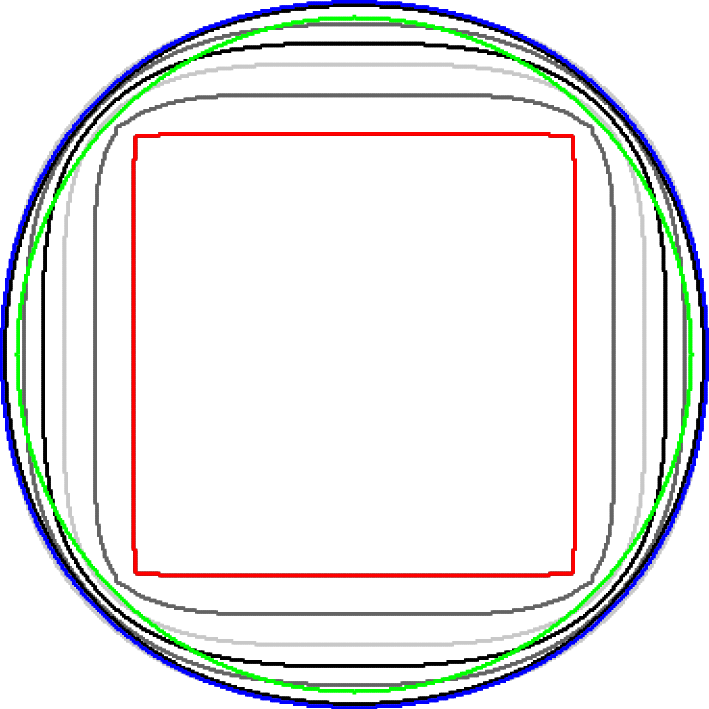
\includegraphics[scale=0.12]{figures/graphcut/with-neighborhood-flow-always-improve/square.png}\\[2em]
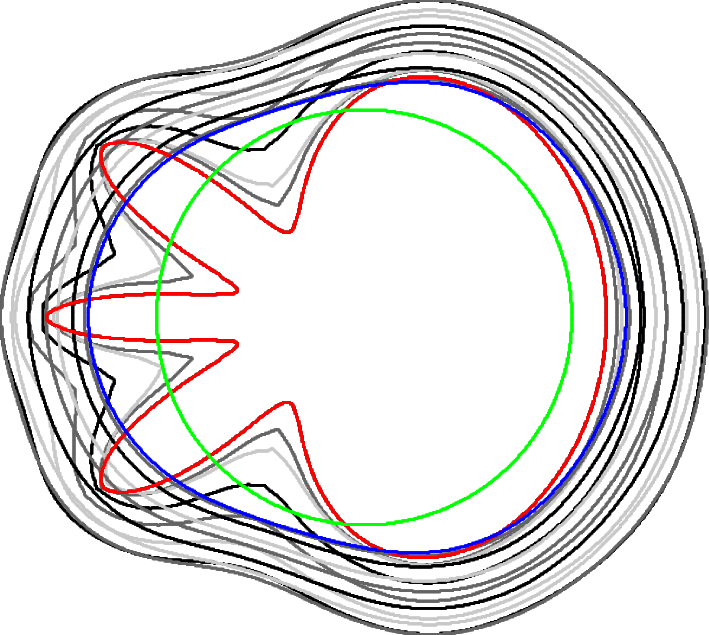
\includegraphics[scale=0.12]{figures/graphcut/with-neighborhood-flow-always-improve/flower.png}\hspace{3em} &
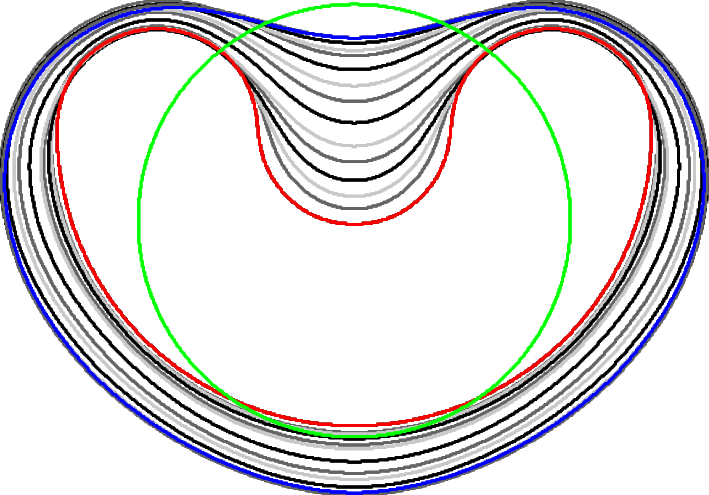
\includegraphics[scale=0.12]{figures/graphcut/with-neighborhood-flow-always-improve/bean.png}
\end{tabular}}
%
%
\only<2>{
\begin{tabular}{cc}
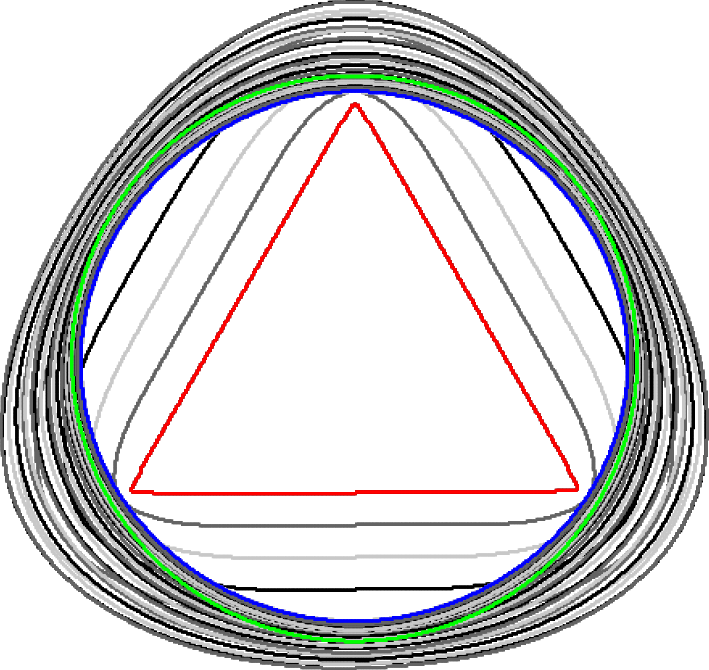
\includegraphics[scale=0.12]{figures/graphcut/with-neighborhood-flow/radius_16/triangle.png}\hspace{3em} &
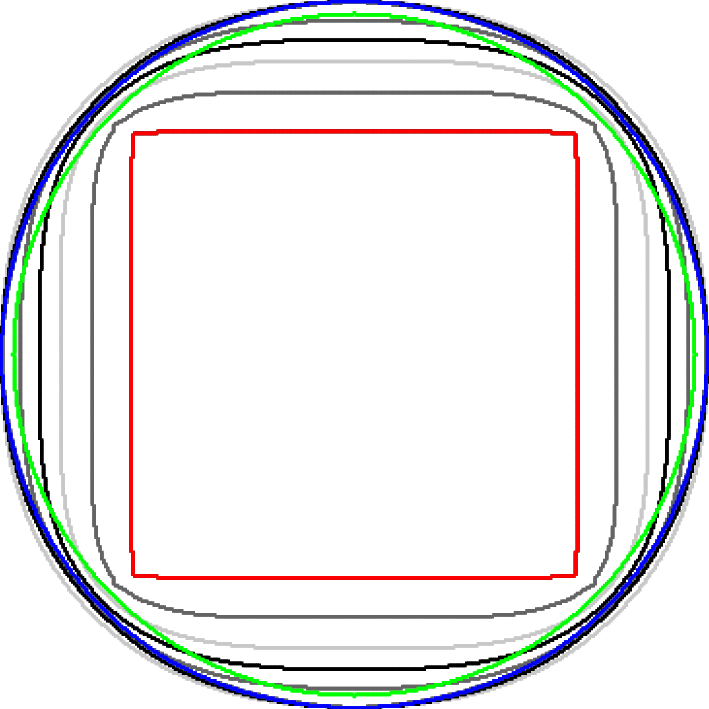
\includegraphics[scale=0.12]{figures/graphcut/with-neighborhood-flow/radius_16/square.png}\\[2em]
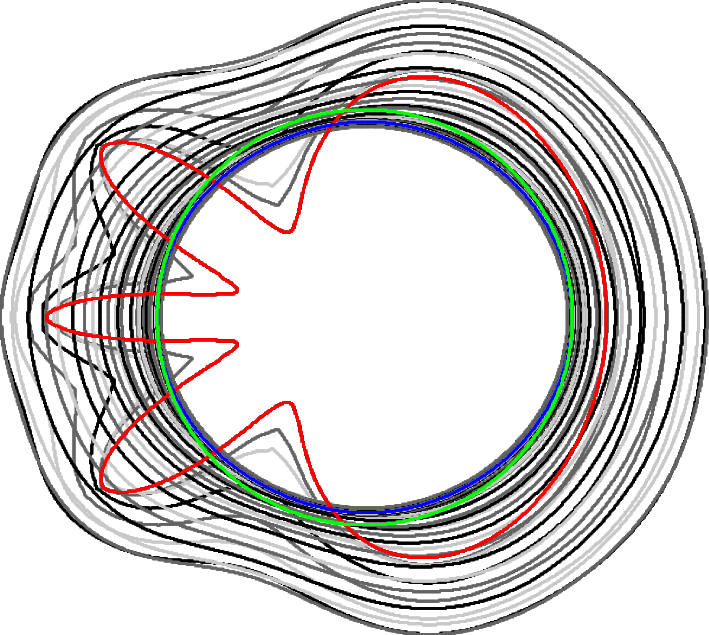
\includegraphics[scale=0.12]{figures/graphcut/with-neighborhood-flow/radius_16/flower.png}\hspace{3em} &
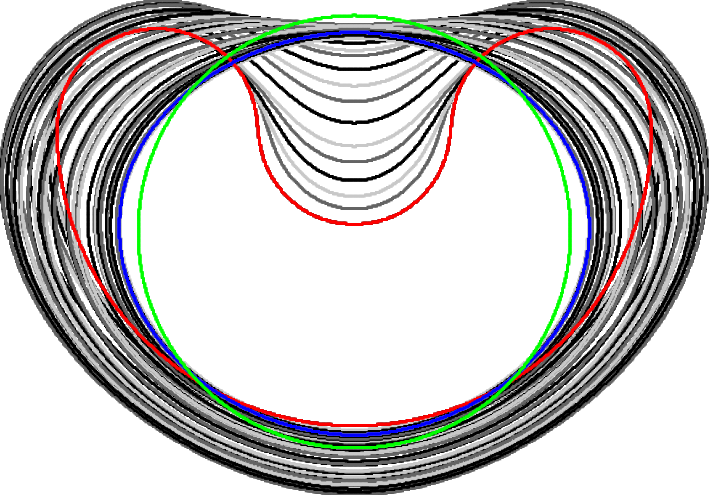
\includegraphics[scale=0.12]{figures/graphcut/with-neighborhood-flow/radius_16/bean.png}
\end{tabular}}
\end{frame}

\begin{frame}
{Elastica minimization via graph-cuts}
{Shape evolution with $a$-probe set}

\begin{minipage}{0.25\textwidth}
\center
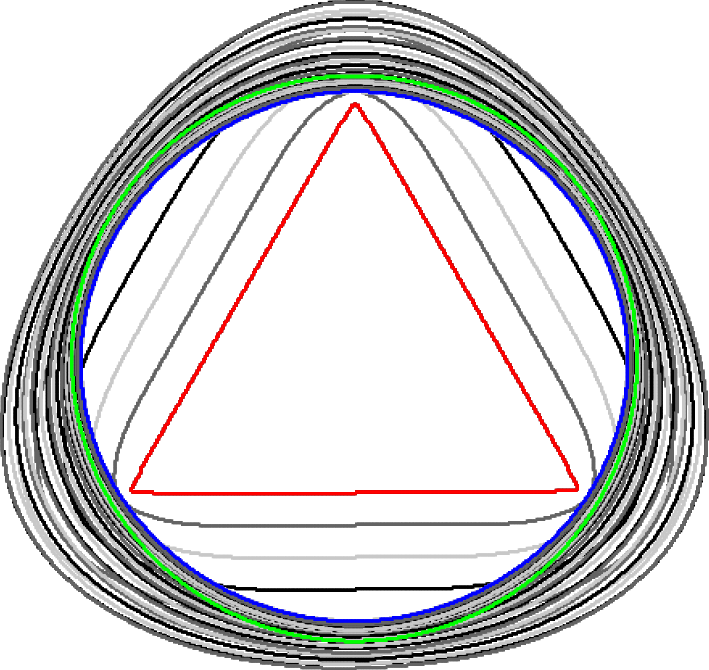
\includegraphics[scale=0.06]{figures/graphcut/with-neighborhood-flow/radius_16/triangle.png}\\[1em]
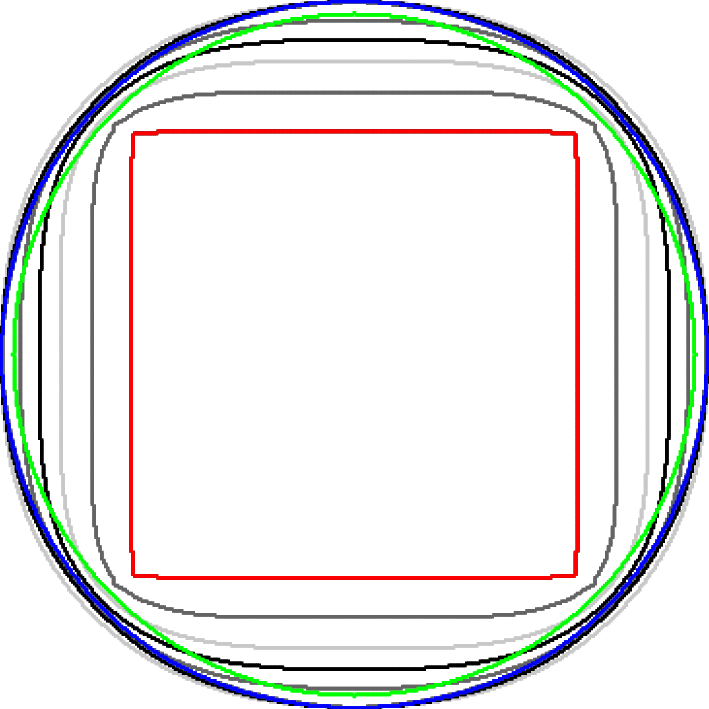
\includegraphics[scale=0.06]{figures/graphcut/with-neighborhood-flow/radius_16/square.png}\\[1em]
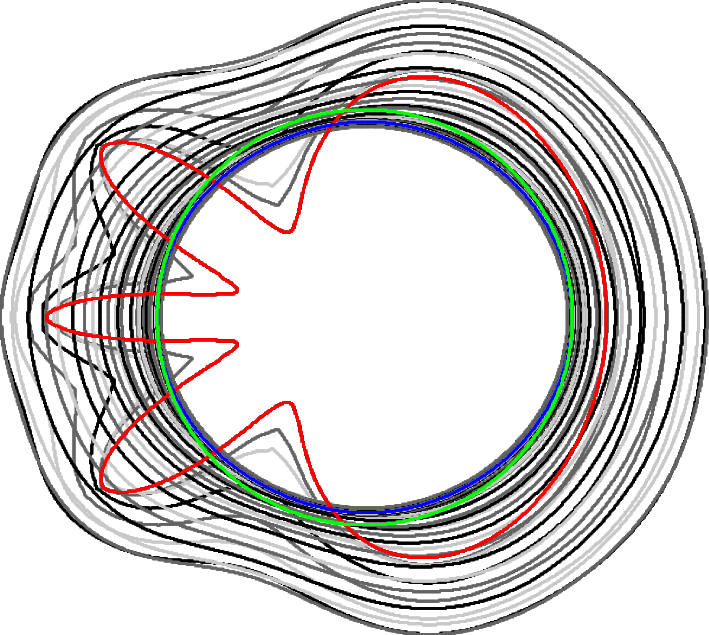
\includegraphics[scale=0.06]{figures/graphcut/with-neighborhood-flow/radius_16/flower.png}\\[1em]
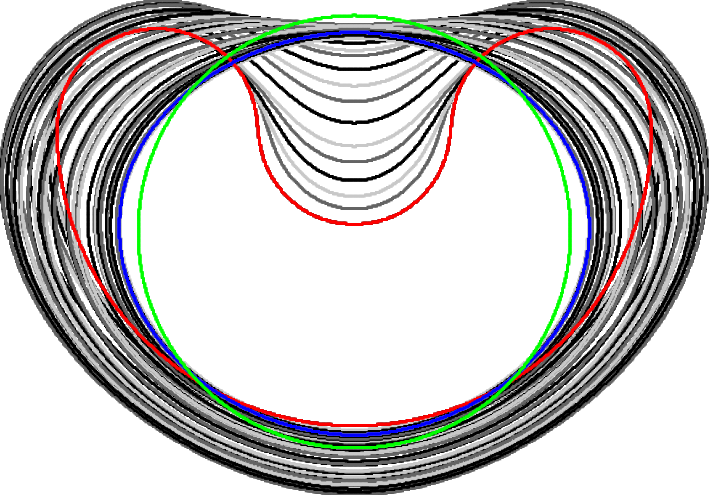
\includegraphics[scale=0.06]{figures/graphcut/with-neighborhood-flow/radius_16/bean.png}
\end{minipage}%
%
%
\begin{minipage}{0.74\textwidth}
\center
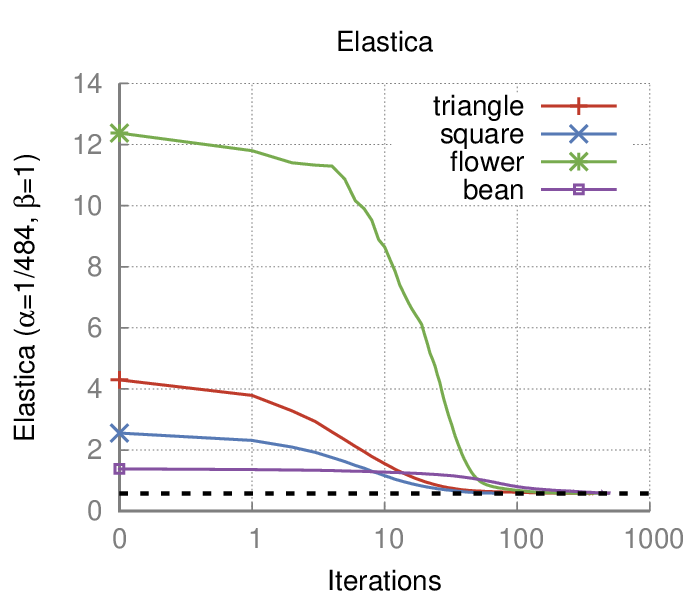
\includegraphics[scale=0.18]{figures/graphcut/with-neighborhood-flow/plots/elastica.png}\\
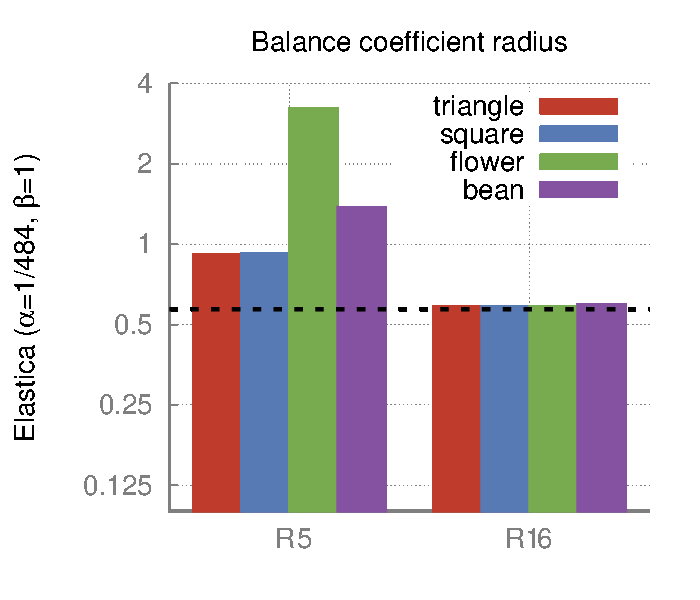
\includegraphics[scale=0.18]{figures/graphcut/with-neighborhood-flow/plots/bars.png}
\end{minipage}
\end{frame}

\begin{frame}
{Elastica minimization via graph-cuts}
{Contour correction}

\begin{minipage}{0.5\textwidth}
\center
\only<1>{
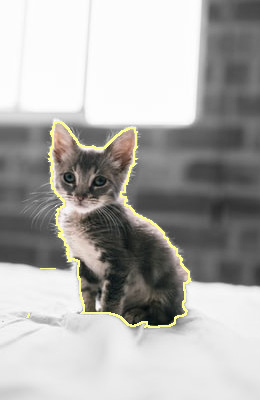
\includegraphics[scale=0.45]{figures/graphcut/contour-correction/cat/gc-seg.png}

Initial segmentation

}%
\only<2>{
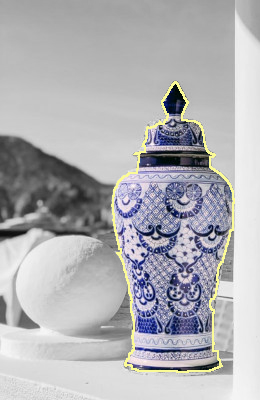
\includegraphics[scale=0.45]{figures/graphcut/contour-correction/vase/gc-seg.png}

Initial segmentation

}%
\only<3,4>{
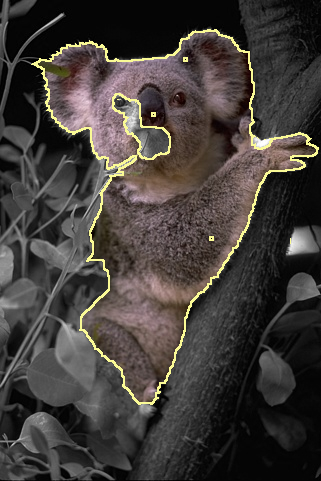
\includegraphics[scale=0.4]{figures/graphcut/contour-correction/coala/gc-seg.png}

Initial segmentation

}%
\end{minipage}%
\begin{minipage}{0.5\textwidth}
\center
\only<1>{
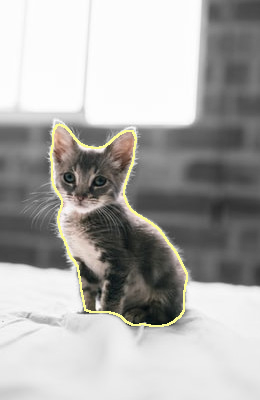
\includegraphics[scale=0.45]{figures/graphcut/contour-correction/cat/corrected-seg.png}

$0.825s$ ($3$ it)

}%
\only<2>{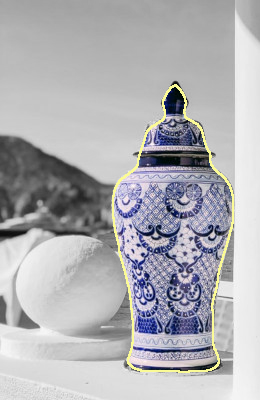
\includegraphics[scale=0.45]{figures/graphcut/contour-correction/vase/corrected-seg.png}

$0.746s$ ($3$ it)

}%
\only<3>{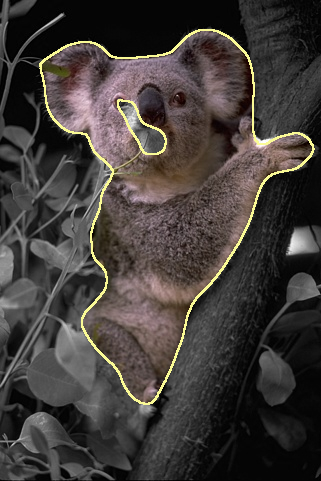
\includegraphics[scale=0.4]{figures/graphcut/contour-correction/coala/5it.png}

$1.1s$ ($3$ it)

}%
\only<4>{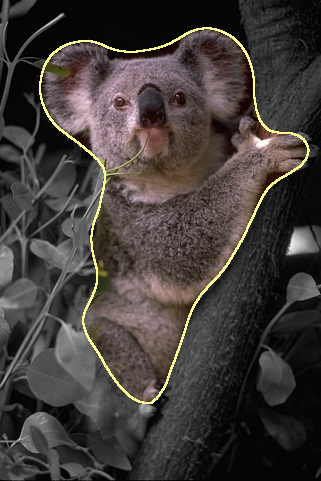
\includegraphics[scale=0.4]{figures/graphcut/contour-correction/coala/30it.png}

$10s$ ($30$ it)

}%
\end{minipage}%

\end{frame}

\begin{frame}
{Elastica minimization via graph-cuts}
{Contour completion}

\begin{minipage}[t][0.47\textheight]{1\textwidth}
\center
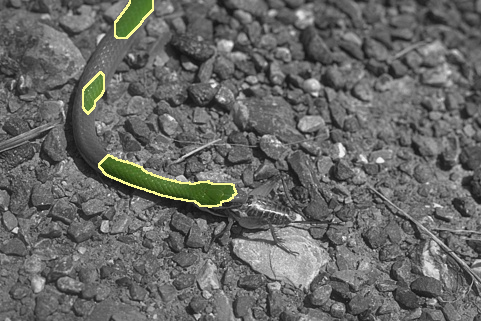
\includegraphics[scale=0.28]{figures/graphcut/contour-completion/green-snake/gc-seg.png}

Initial segmentation

\end{minipage}
\vspace{1em}
\begin{minipage}[t][0.47\textheight]{1\textwidth}
\center
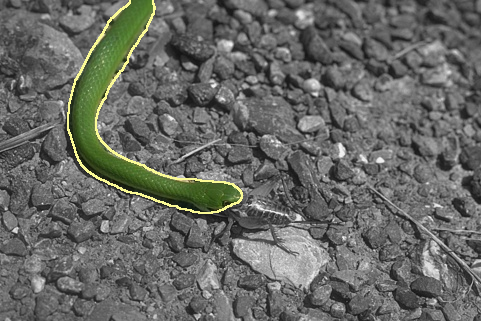
\includegraphics[scale=0.28]{figures/graphcut/contour-completion/green-snake/corrected-seg.png}

$17s$ ($62$ it)

\end{minipage}


\end{frame}
